\newpage
\thispagestyle{sectioned}
\chapter{Metodología}

\section{Diseño Guiado Por Objetivos}

Para elaborar el diseño de la aplicación, nos hemos basado en la metodología del Diseño Guiado por Objetivos, una metodología que implementa el proceso de la ingeniería de la usabilidad propuesta por Alan Cooper \cite{ref:bookAlanCooper}. Este proceso constará de las siguientes fases:

1. Investigación

2. Modelado

3. Definición de requisitos

4. Framework de diseño

Insistimos una vez más en que nos hemos basado en esta metodología para seguir el proceso del diseño de la aplicación. Por lo que no cumpliremos esta metodología al 100% de sus fases debido a preferencias personales.

Una vez puesta en marcha la intención y los principales objetivos de la aplicación, procedimos a entrevistarnos con gente para realizar una investigación sobre las necesidades prácticas de la idea. Y por otra parte verificar los prototipos que anteriormente habíamos realizado. El tipo de persona con el que nos entrevistamos debía de estar relacionado con el mundo político, pues debía de manejar diferentes conceptos y mostrar cierto interés por la participación ciudadana en la política.

A continuación detallamos las entrevistas que realizamos en la investigación:

\section{Investigación}
La intención fundamental de la aplicación es llevar los programas electorales a los bolsillos de los ciudadanos. Vivimos en una sociedad digital, donde cada vez son más las personas que utilizan los teléfonos inteligentes para realizar todo tipo de tareas en su vida cotidiana.

En los últimos años las diferentes formaciones políticas han subido sus programas electorales a un documento en formato pdf que estaba disponible en su página web. Este documento generalmente extenso, no es un medio fácil de divulgar y mostrar a la ciudadanía. Por ello pensamos que una aplicación que pudiera visualizar las principales secciones de los programas políticos, podría ser especialmente útil para acercar los programas a los electores.

Llegando a crear un espacio donde poder informase sobre las distintas ofertas electorales, debatir las propuestas que propone cada formación política reducido en una aplicación que podremos consultar en cualquier momento.

Además de esto, crearemos un portal de propuestas ciudadanas. Donde los usuarios podrán visualizar las propuestas por temas, visualizarlas en función de unos datos, y tener la posibilidad de crear nuevas propuestas ciudadanas. Existen multitud de portales donde la ciudadanía puede expresar su opinión, pero creemos que la integración de una aplicación donde puedan situarse los partidos políticos y la actividad ciudadana, genera una nueva visión de trabajar la política en los medios sociales.

\subsection{Entrevista con Labodemo}
Tuvimos la oportunidad de establecer una conversación con dos miembros de Labodemo \cite{ref:labodemo}, en la que aprovechamos la oportunidad de mostrarles la aplicación que estábamos desarrollando. Ambos tenían experiencia en el desarrollo de plataformas de participación ciudadana en internet y nuevas tecnologías. Además fueron los responsables del desarrollo de los portales de participación del partido político Podemos y la candidatura ciudadana de unidad popular Ahora Madrid.

Limitarnos a mostrar las diferentes secciones de cada programa les resultó útil. Aunque no suficiente como para atraer a una cantidad considerable de usuarios. Antes de hablar con ellos, habíamos planteado desarrollar propuestas colaborativas en tiempo real aprovechando Wave. Pero no comprendieron la libertad de dar al usuarios la creación de propuestas colaborativas en tiempo real.

Dándole una vuelta al desarrollo de las propuestas de la aplicación, nos sugirieron que para atraer a usuarios a utilizar nuestra aplicación, deberíamos dejar cierta libertad a colectivos sociales. Por ejemplo, un grupo de animalistas debería tener un “espacio” en la aplicación donde poder crear sus propias propuestas, e incluso hacer comparativas personalizadas de lo que proponen los diferentes programas sobre los animales. Así surgirían propuestas y comparativas divididas por colectivos que abarcarían diferentes temáticas. Un usuario poco activo podría buscar un colectivo de profesores porque resulta ser su profesión, y ver las propuestas que se llevan a cabo o visualizar una comparativa respecto las medidas de educación de los diferentes programas políticos.

Organizar estas propuestas no sería tarea sencilla. En un principio se propuso como diferentes temas que puede tener un foro, en forma de post. Más tarde llegamos a la conclusión de que sería más cómodo para los colectivos dar la libertad de crear sus propios hilos, y en cada uno de ellos publicar las propuestas relacionadas con su colectivo.

Por último insistieron mucho en el tema de las comparativas. Sería de gran utilidad que la aplicación tuviera una parte de comparativas en la que los usuarios pudieran comparar los programas políticos en vez de leerlos sección por sección. Resultaría de gran interés a un autónomo visualizar las medidas que proponen los diferentes partidos políticos para los autónomos. Pero estas comparativas no podría realizarlas cualquiera, por lo que deberían realizarlas periodistas o expertos que hubieran realizado algún tipo de comparativa similar anteriormente. Nos sugirieron contactar con periodistas o colectivos que hubieran publicado algún tipo de comparativa en cuando a programas o medidas, para obtener algún tipo de ayuda o consejo a seguir.

\subsubsection{Conclusión}
La reunión con dos de los miembros de Labodemo resultó de gran interés. Pues desde que decidimos la idea que íbamos a implementar, nunca habíamos puesto en práctica la aplicación o al menos no la habíamos verificado con el “mundo real”.

Los integrantes de Labodemo eran expertos en desarrollo de portales de participación ciudadana. Y sobre todo estaban muy familiarizados con el uso común que les suele dar la gente a este tipo de aplicación. Por lo que sabían determinar las claves para que una aplicación tuviera un movimiento considerable de usuarios desde el comienzo.

El tema de visualizar los programas políticos no les gustó demasiado. Expusieron que un ciudadano de a pie, no iba a molestarse en leer los programas políticos. Bien porque no los entienda o porque les resulte aburridos. Ellos argumentaban que los colectivos sociales serían los usuarios más activos en nuestra aplicación, por lo que debíamos enfocar más el desarrollo hacia la partición ciudadana y el uso de propuestas o comparativas por colectivo.

Tras esta reunión decidimos replantear la aplicación en base a los consejos que obtuvimos con la reunión de Labodemo. Incluimos las propuestas como parte de nuestra aplicación y empezamos a pensar la forma de colaborar de grupos y colectivos. También intentamos contactar con colectivos y personas interesadas en el desarrollo de la aplicación. Finalmente, conseguimos concretar una entrevista con Javier de la Cueva \cite{ref:jdelacueva}.

\subsection{Entrevista con Javier de la Cueva}

La entrevista con Javier de la Cueva resultó más que productiva. Ya conocíamos a Javier de la Cueva de algunas conferencias que impartió en la facultad. Javier de la Cueva es abogado y doctorado en Filosofía, está especializado en tenas relacionados con tecnología, internet y propiedad intelectual. Además, en sus últimas conferencias Javier habla sobre acciones micropolíticas \cite{ref:manualCiberactivista}. Estas acciones definen la capacidad que tiene las ciudadanía para realizar aportaciones a la sociedad, el estado o el gobierno que favorezcan la participación ciudadana en una democracia participativa.

Representar los programas electorales en una aplicación móvil resultó más que interesante a parte de necesario para la sociedad actual. Si bien casi nadie hace el esfuerzo de visualizar un programa electoral en pdf, utilizar una herramienta que facilita el acceso al programa por secciones podría ser una nueva forma de incentivar la participación política. 

Además se comentó la posibilidad de desarrollar una pequeña hemeroteca de programas electorales. De forma que cualquiera pudiera consultar los programas de los gobiernos pasados y comprobar si se cumplieron los objetivos del programa. Pero si en algo nos insistió Javier, fue en categorizar el contenido de la aplicación. Un usuario que no tenga muchos conocimientos sobre diversos temas de la sociedad, se encontraría más cómodo si pudiera visualizar las diferentes partes de un programa o las propuestas ciudadanas, por categorías o temas generales. Ya que dejando libertad a que los usuarios pudieran crear categorías personalizadas podría ser algo negativo para usuarios inexpertos o poco adentrados en temas específicos.

Por último, centrándonos en las propuestas ciudadanas, surgió la idea de elaborar propuestas que tuvieran una especificación concreta. Es decir, a parte de tener una idea de propuesta y redactarla, esta propuesta debería ir acompañada de los recursos que serían necesarios y sobre todo cómo se llevaría a cabo de una forma aproximada. También resultaría interesante definir un pequeño presupuesto de lo que conllevaría realizar la propuesta o cómo se podría financiar. Así evitaríamos una elaboración de propuestas más real, evitando un listado de propuestas infinito sin planterase cómo se llevarían a cabo o cómo se financiarían.

\subsubsection{Conclusión}

Javier trató de abrirnos un poco más la mente, para plantearnos ideas que no están representadas en la sociedad. En la actualidad encontramos diversas plataformas de participación ciudadana que acaban convirtiéndose en un foro. Para evitar caer en esto, debíamos innovar algo más para volver a repetir esto, debíamos de intentar desarrollar nuevas formas de participación.

Clasificar las secciones de un programa así como también las propuestas ciudadanas en diferentes categorías y temas era algo que descartamos en un principio, pero nuevamente volvió a llamar nuestro interés. Aunque para dar cierta libertad, podríamos incluir la posibilidad de crear categorías personalizadas o ir añadiendo categorías semanalmente.

\section{Modelado}

En esta fase definiremos el tipo de persona que interactuará con nuestra aplicación. Para ello hemos identificado dos tipos de personas primarias:

\textbf{- Activista social, 16 años en adelante}

\underline{Actividad:}

\begin{itemize}
\item Estudia, trabaja o realiza otras actividades de voluntariado.
\item Frecuenta asambleas, participa en diferentes movimientos sociales y está al día de la actualidad política.
\item Utiliza redes sociales para comunicarse con otros colectivos, acudir a asambleas, promover ideas u otras actividades relacionadas con la política y el activismo social.
\end{itemize}

\underline{Otros:}

\begin{itemize}
\item Desconoce las ideas que proponen algunos partidos 
\item Le gusta aportar nuevas soluciones a la sociedad.
\end{itemize}

\textbf{- Ciudadano de a pie, 18 años en adelante}

\underline{Actividad:}

\begin{itemize}
\item Estudia, trabaja o realiza otras actividades de voluntariado.
\item Es distante al mundo de la política, concibe ciertos temas pero no los conoce en profundidad.
\item Visita diferentes medios de comunicación para enterase de la actualidad.
\item Utiliza redes sociales para compartir contenidos con sus amigos o establecer nuevas amistades.
\end{itemize}

\underline{Otros:}

\begin{itemize}
\item Desconoce por completo los programas electorales. 
\item Tiene cierta indecisión a la hora de acudir a las urnas, no sabe que propone cada partido.
\end{itemize}

\section{Definición de Requisitos}
En esta sección se definirán los posibles escenarios que puedan surgir en la aplicación:

\textbf{Escenario I}

Se acercan las elecciones municipales y Juan aún no ha decidido a qué partido va dar su voto. No conoce las propuestas que ofertan los partidos a la ciudadanía y tampoco se fía mucho de lo que dicen los medios de comunicación.

Juan coge su móvil y visualiza los diferentes programas electorales por categoría, seleccionando la categoría de educación que es la que más le afecta a él personalmente. La aplicación le muestra un listado de las secciones donde lso diferentes partidos hablan de las medidas que van a tomar en torno a la educación.

\underline{Requisitos:}

\begin{enumerate}
\item Visualizar (acción) las diferentes categorías (objeto), para ver las secciones de los programas de una determinada categoría (contexto).
\item Mostrar(acción) un listado de todas las secciones de los programas de los partidos  políticos (objeto) en función de la categoría seleccionada por el usuario (contexto).
\end{enumerate}

\textbf{Escenario II}

Pablo es un empleado sanitario de Hospital Clínico de Madrid preocupado por la gestión de los hospitales públicos. Parece que la situación no está muy controlada, por lo que quisiera saber que propuestas o alternativas propone la ciudadanía para mejorar la situación actual.

A través de su móvil puede explorar las diferentes propuestas por categorías. Eligiendo la categoría de sanidad, le aparece un listado de las últimas propuestas desarrolladas por la ciudadanía.

\underline{Requisitos:}

\begin{enumerate}
\item Mostrar (acción) las diferentes categorías (objeto), para visualizar las propuestas ordenadas por la categoría seleccionada (contexto).
\item Visualizar (acción) el listado de propuestas (objeto), clasificados por la categoría seleccionada por el usuario (contexto).
\end{enumerate}

\textbf{Escenario III}

\underline{Requisitos:}

\begin{enumerate}
\item
\item
\item
\end{enumerate}

\textbf{Escenario IV}

\underline{Requisitos:}

\begin{enumerate}
\item
\item
\item
\end{enumerate}

\textbf{Escenario V}

\underline{Requisitos:}

\begin{enumerate}
\item
\item
\item
\end{enumerate}

\section{Framework de diseño}

En esta sección detallaremos todos los aspectos relacionados con el aspecto visual de la aplicación. Detallaremos los prototipos desarrollados en papel, algunos prototipos intermedios y el prototipo final de la aplicación.

\subsection{Metodología}

En una primera fase procedimos a realizar una serie de prototipos rápidos a papel para visualizar una interacción de las principales características de la aplicación. A continuación llevamos estas ideas a papel nuestra aplicación desarrollada en Android. Obteniendo un prototipo de media-alta fidelidad sobre la funcionalidad de la aplicación.

Cuando quisimos añadir nuevas características volvimos a desarrollar nuevos prototipos a papel de las pantallas a desarrollar. Por último, se desarrollaron las nuevas pantallas y se refinaron las anteriores para llegar a un prototipo de alta fidelidad o una versión alpha de la aplicación.

\subsection{Prototipos a papel}

Meter las fotos de los prototipos a papel y comentarlos.

\subsection{Prototipos intermedios}

La aplicación pretende llevar las principales partes de los programas electorales de los partidos que se presenten a las elecciones. Por tanto, cualquier usuario podrá visualizar el apartado que desee consultar de cualquier partido político. Siendo esta la forma menos amigable de leerlo, se utilizarán distintas formas para compartir o divulgar determinadas secciones más populares.

Al inicio de la aplcación, mostrará una lista de las secciones de los programas más valoradas, más debatidas, peor valoradas e incluso las más incomprendidas. Por tanto creemos que puede ser una forma de acercar aquellas secciones más populares de forma más eficaz, al contrario que tener que consultar una determinada página dentro de un extenso pdf.

\begin{figure}[H]
\centering
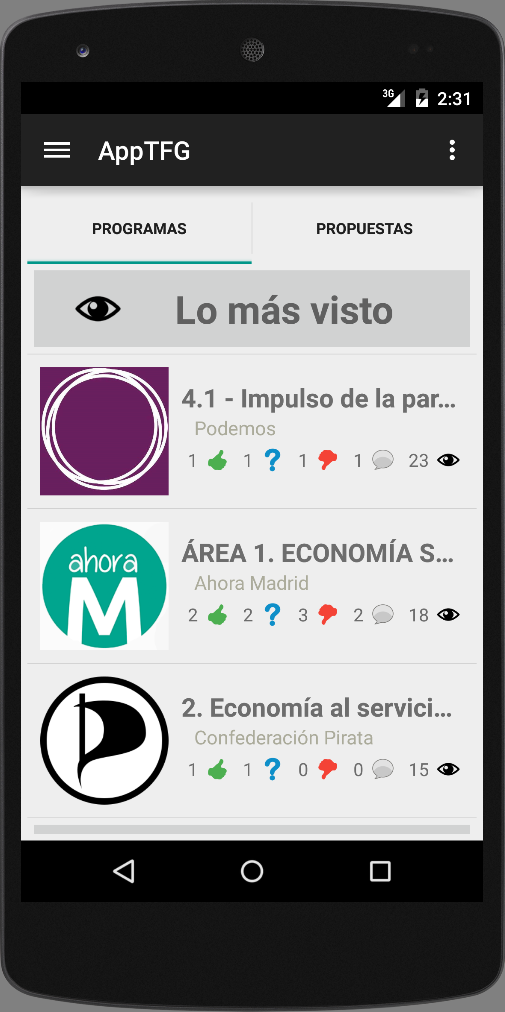
\includegraphics[keepaspectratio, scale=0.5]{Media/Captures/captTopSections.png}
\caption{Vista principal de secciones}
\label{fig:captTopSections}
\end{figure}

Dentro de cada sección podemos visualizar el contenido de la sección a la que referencia el programa, y tendremos la opción de valorarla de forma positiva o negativa. También añadimos la posibilidad de indicar que no se ha entendido la sección. Pues a la hora de leer una propuesta de gobierno ubicada en una sección del programa, bien nos puede gustar, disgustar o simplemente no haber entendido la idea y por ello no votarla de forma positiva o negativa.

\begin{figure}[H]
\centering
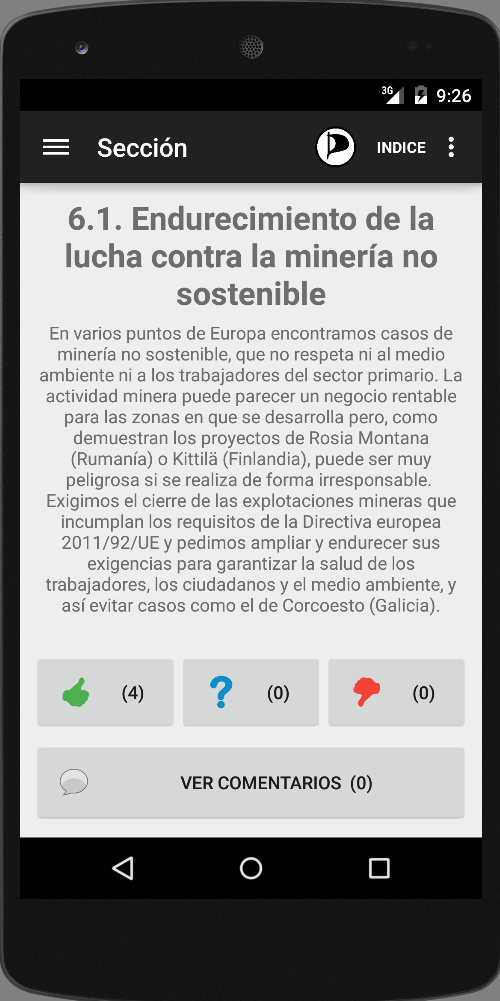
\includegraphics[keepaspectratio, scale=0.5]{Media/Captures/section.png}
\caption{Visualizando una sección}
\label{fig:captSection}
\end{figure}

Sin olvidarnos de la parte social, en cada sección podemos hacer comentarios para intentar debatir las ideas fundamentales que propone la sección. O incluso hacer referencia a una determinada frase o párrafo.

\subsection{Prototipo final}

\subsection{Usabilidad}

Hablar de las reglas de oro, principios de diseño,...
